\makeatletter
\def\input@path{{../../}}
\makeatother
\documentclass[../../main.tex]{subfiles}

\graphicspath{
	{../../img/}
	{../img/}
	{img/}
}

\begin{document}

% \section{Эйлеровы интегралы первого и второго рода}

\section{Гамма-функция Эйлера}

Эйлеровым интегралом второго рода или гамма-функцией называется
\begin{equation}
\label{lec13:1}
\Gamma(a) = \int\limits_0^{+\infty}e^{-x}x^{a-1}dx
\end{equation}

\[
	f(x, a) = e^{-x}x^{a-1}
\]  непрерывное на $\forall x > 0, \forall a \in \R$
\\
$
	x \implies +0; f(x, a) \sim [e^{-1} \to 1] \sim \frac{1}{x^{1-a}}
	\Gamma(a) = \int\limits_0^1e^{-x}x^{a-1}dx + \int_0^{+\infty}e^{-x}x^{a-1}dx
$
\\
$
1) x \to + 0; f(x, a) \underset{k \to +0}\sim \left[ e^{-x} 
\underset{x \to +0} \to 1 \right] \sim \frac{1}{x^{1-a}}
$
\\
$
	2) x \to +\infty; 
	0 \le f(x, a) = \dfrac{x^{a+1}}{e^x} \cdot \dfrac{1}{x^2} \le \dfrac{c}{x^2}, 
	c=const \ge 0;
$

Особенность \eqref{lec13:1}, $\Gamma(a) = \int\limits_0^1 e^{-x} x^{a-1} dx +
\int\limits_1^{+\infty} e^{-x} x^{a-1} dx $ - 
Первый интеграл~--- НИЗОП-2, второй~--- НИЗОП-1. 
Первое слагаемое сходится, когда \begin{equation}
	\label{lec13:2}
	1 - a < 1 \implies a > 0
\end{equation}

$\int\limits_1^{+\infty}\dfrac{c}{x^2}dx$~--- сходится по степенному признаку.

Второе слагаемое НИЗОП-1 также сходится по признаку сравнения 1.
\\\\
Область существования(сходимости) для \eqref{lec13:1} будет $\forall a \in ]0, 
+\infty[$.
\\\\
Нетрудно получить, что оба слагаемых в \eqref{lec13:2} в полученной области 
сходятся по Вейерштрассу локально равномерно:
\[
\Gamma(a) \overset{\forall \left[ \alpha, \beta \right] \in (0, 
+\infty)}{\rightrightarrows}
\]

В области сходимости~--- непрерывная функция от а.

Учитывая, что для \eqref{lec13:2}
$
\exists f'_a(x, a) = (e^{-x} x^{a-1})'_a = e^{-x}x^{a-1} \ln x$ 
непрерывна$\forall x>0,\forall a >0.
$

\[
\int\limits_0^{+\infty} e^{-x} x^{a-1} \ln x dx
\overset{\forall \left[ \alpha, \beta \right] \in (0, 
	+\infty)}{\rightrightarrows}
\]

$
\exists \Gamma'(a) = \int\limits_0^{+\infty} (e^{-x} x^{a-1})'_a dx = 
\int\limits_0^{+\infty} e^{-x} x^{a-1} \ln x dx 
$
непрерывна
$\forall a > 0$

Аналогичным образом по индукции $\forall k \in \N$

$
\Gamma^{(k)}(a) = \ldots = \int\limits_0^{+\infty} e^{-x} x^{a-1} \ln x dx 
$

$
\forall x \in N_0 \implies \exists f^{(k)}_a = \cdots = 
\int\limits_0^{+\infty} e^x x^{a-1} \ln^k x dx 
$

Гамма-функция бесконечно число раз непрерывно дифференцируема.
При этом, т.~к. $\Gamma'(a) = \int\limits_0^{+\infty} e^{-x} x^{a-1} \ln^2 x 
dx \ge 
0$,
то график для Г(а) будет выпуклым вниз. Имеем
$
\Gamma(1) = \int\limits_0^{+\infty} e^{-x} dx = [-e^{-x}]^{+\infty}_0 = 1
\\
\Gamma(2) = \int\limits_0^{+\infty} e^{-x} \alpha dx = 
- \int\limits_0^{+\infty} x d(e^{-x}) = 
xe^{-x}|^{+\infty}_0 + \int\limits_0^{+\infty} e^{-x} dx = 
0 + 1 = 1
\\
\exists a_0 \in (1, 2) \implies \Gamma'(a_0) = 0$, т.~е. $a_0$~--- 
стационарная 
точка~--- точка минимума.

Приближенное вычисление $a_0 \simeq 1,462$

$\Gamma(a_0) = \Gamma_{min} \simeq 0.886$

В результате график

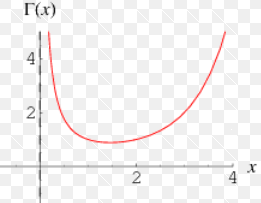
\includegraphics[scale = 1]{../../img/lec13_1}


Интегрирование по частям имеем:
$
\Gamma(a) = \int\limits_0^{+\infty} e^{-x} d(\dfrac{x^a}{a}) =
 \dfrac{e^{-x}x^a}{a} |^{+\infty}_0 - \int\limits_0^{+\infty} \frac{x^a}{a} 
 d(e^{-x}) = 
 \frac{1}{a} \int\limits_0^{+\infty} e^{-x} x^a dx = \frac{\Gamma(a+1)}{a}
\\
\Gamma(a) = \frac{\Gamma(a+1)}{a}
\\
\Gamma(0) \simeq \frac{\Gamma(1)}{a} = \dfrac{1}{a}
$
a=0~--- асимптота

Формула понижения
\\
$
\Gamma(a+1) = a\Gamma(a), \forall a > 0
\\
\Gamma(1) = 1
\\
\forall n \in \N
\\
\Gamma(n) = (n-1)\Gamma(n-1) = \cdots = (n-1) \cdot \ldots \cdots 2 \cdot 1 
\Gamma(1) = (n-1)!
$

\begin{equation}
\label{lec13:4}
\Gamma(n) = (n-1)!,  \forall n \in \N
\end{equation}

\eqref{lec13:4}~--- гамма-функция~--- обобщение факториала.. 
Использование функции

$
a = n + \frac{1}{2}, n \in \N
\\
\Gamma(n + \frac{1}{2}) = (n - \frac{1}{2})\Gamma(n-\frac{1}{2})=\ldots=
(n-\frac{1}{2})(n-\frac{3}{2})\ldots\frac{3}{2}\frac{1}{2}\Gamma(\frac{1}{2}) 
= 
\frac{(2n-1)!!}{2^n}\Gamma(\frac{1}{2})
$
Используем интеграл Эйлера-Пуассона:
\\
$
\Gamma(\frac{1}{2})= \int\limits_0^{+\infty} e^{-x} x^{-\frac{1}{2}} dx = [] = 
\int\limits_0^{+\infty} e^{-t^2} t^{-1} 2t dt^2 = 2 \int\limits_0^{+\infty} 
e^{-t^2} dt 
= 2 \frac{\sqrt{\pi}}{2} = \sqrt{\pi}
$

\begin{equation}
	\label{lec13:5}
	\begin{cases}
		\Gamma(n+\frac{1}{2}) = \frac{(2n-1)!!}{2^n} \sqrt{\pi}, \forall n \in \N \\
		\Gamma(\frac{1}{2}) = \sqrt{\pi}
	\end{cases}
\end{equation}

\section{Бета-функция Эйлера}
Бета-функцией Эйлера или эйлеровым интегралом второго рода называется
\begin{equation}
	\label{lec13:6}
	B(a, b) = \int\limits_0^1x^{a-1}(1-x)^{b-1}dx
\end{equation}

\begin{equation}
	\label{lec13:7}
	B(a, b) = \int\limits_0^{\frac{1}{2}} 
	x^{a-1} (1-x)^{b-1}dx + \int\limits_{\frac{1}{2}}^{1} 
	x^{a-1}(1-x)^{b-1}dx
\end{equation}


\[1) f(x, a, b) = x^{a-1}(1-x)^{b-1}_{x\to+0} \sim \dfrac{1}{x^{a-1}}\]
Первое слагаемое будет сходится \[ 1 - a < 1 \implies a > 0 \]

\begin{equation}
	2) f(x, a, b) \sim \dfrac{1}{(1-x)^{1-b}}
\end{equation}
Второе слагаемое сходится при области сходимости \[ 1-b < 1 \implies b > 0 \]

В итоге, области сходимости \eqref{lec13:6} будут \[a > 0, b > 0\].
В дальнейшем основные свойства будем получать из свойств Г-функций.
% \eqref{lec10:7}

\begin{thm}[Связь гамма-функции и бета-функции]
	\begin{equation}
	\label{lec13:8}
	\forall a > 0, \forall b>0 \implies B(a, b) = 
	\dfrac{\textup{Г(а)Г(b)}}{\textup{Г(а+b)}}
	\end{equation}
\end{thm}

\begin{proof}
	$\Gamma(a) \stk{lec13:1}= [x=ty, y = \dfrac{x}{t}|^{+\infty}_0, t > 0 - \fix, 
	dx = 
	t dy] = 
	\int\limits_0^{+\infty}e^{-ty}(ty)^{\alpha-1}tdy = t^a 
	\int\limits_0^{+\infty}e^{-ty}y^{\alpha-1}dy$
	\begin{equation}
		\label{lec13:9}
		\dfrac{\Gamma(a)}{t^a}=\int\limits_0^{+\infty}e^{-ty}y^{\alpha-1}dy
	\end{equation}
	
	заменяя в \eqref{lec13:8} $a > 0$ на $a+b > 0$ и $t > 0$ на $(1+t) > 0$, 
	получаем:
	
	\begin{equation}
	\label{lec13:10}
	\dfrac{\Gamma(a+b)}{(1+t)^{a+b}} = \int\limits_0^{+\infty} e^{-(1+t)y} 
	y^{(a+b) - 
	1} dy
	\end{equation}
\end{proof}

\end{document}
